\subsection{Problem in Localization}

\paragraph{}
In this project, we decided to realize the challenge through visual servoing.
That is to say a line tracking by the camera. This type of servoing only
works if the robot has at all times the line to follow in its field of vision. 
But this is not possible since it will very often happen that the robot loses sight of the line. Especially during a turn. So if our car loses sight of the line, we'll have to get it back on the track.


\paragraph{}

\subsection{Robot status estimation}

\paragraph{}
To compensate for this very likely situation, 
we have a control law in place that will be used as soon as the robot loses the line. 
This law of control requires knowledge of the robot's condition.

\begin{figure}[!ht]
    \begin{center}
        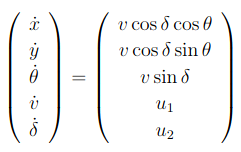
\includegraphics[scale=0.6]{Images/Etat_tricycle.png}
    \end{center}
    \caption{State of the robot}
    \label{fig:State}
\end{figure}

\paragraph{}
Where (x,y) is the position of the robot, $\theta$ is its heading, v its speed and $\delta$ the angle of the front wheels.
To be able to apply a Kalman filter we need a linear state representation of the robot. To make these equations linear, 
we have considered the angle $\theta$ of the robot as an input (since it is given by the inertial unit). 
This removes equation 3. Then we linearized the equation into xhat (xhat being the new state to be determined).xhat consists of x,y, $\theta$, $\delta$. 
The file  available on our github shows the function of this Kalman filter.


\begin{figure}[!ht]
    \begin{center}
        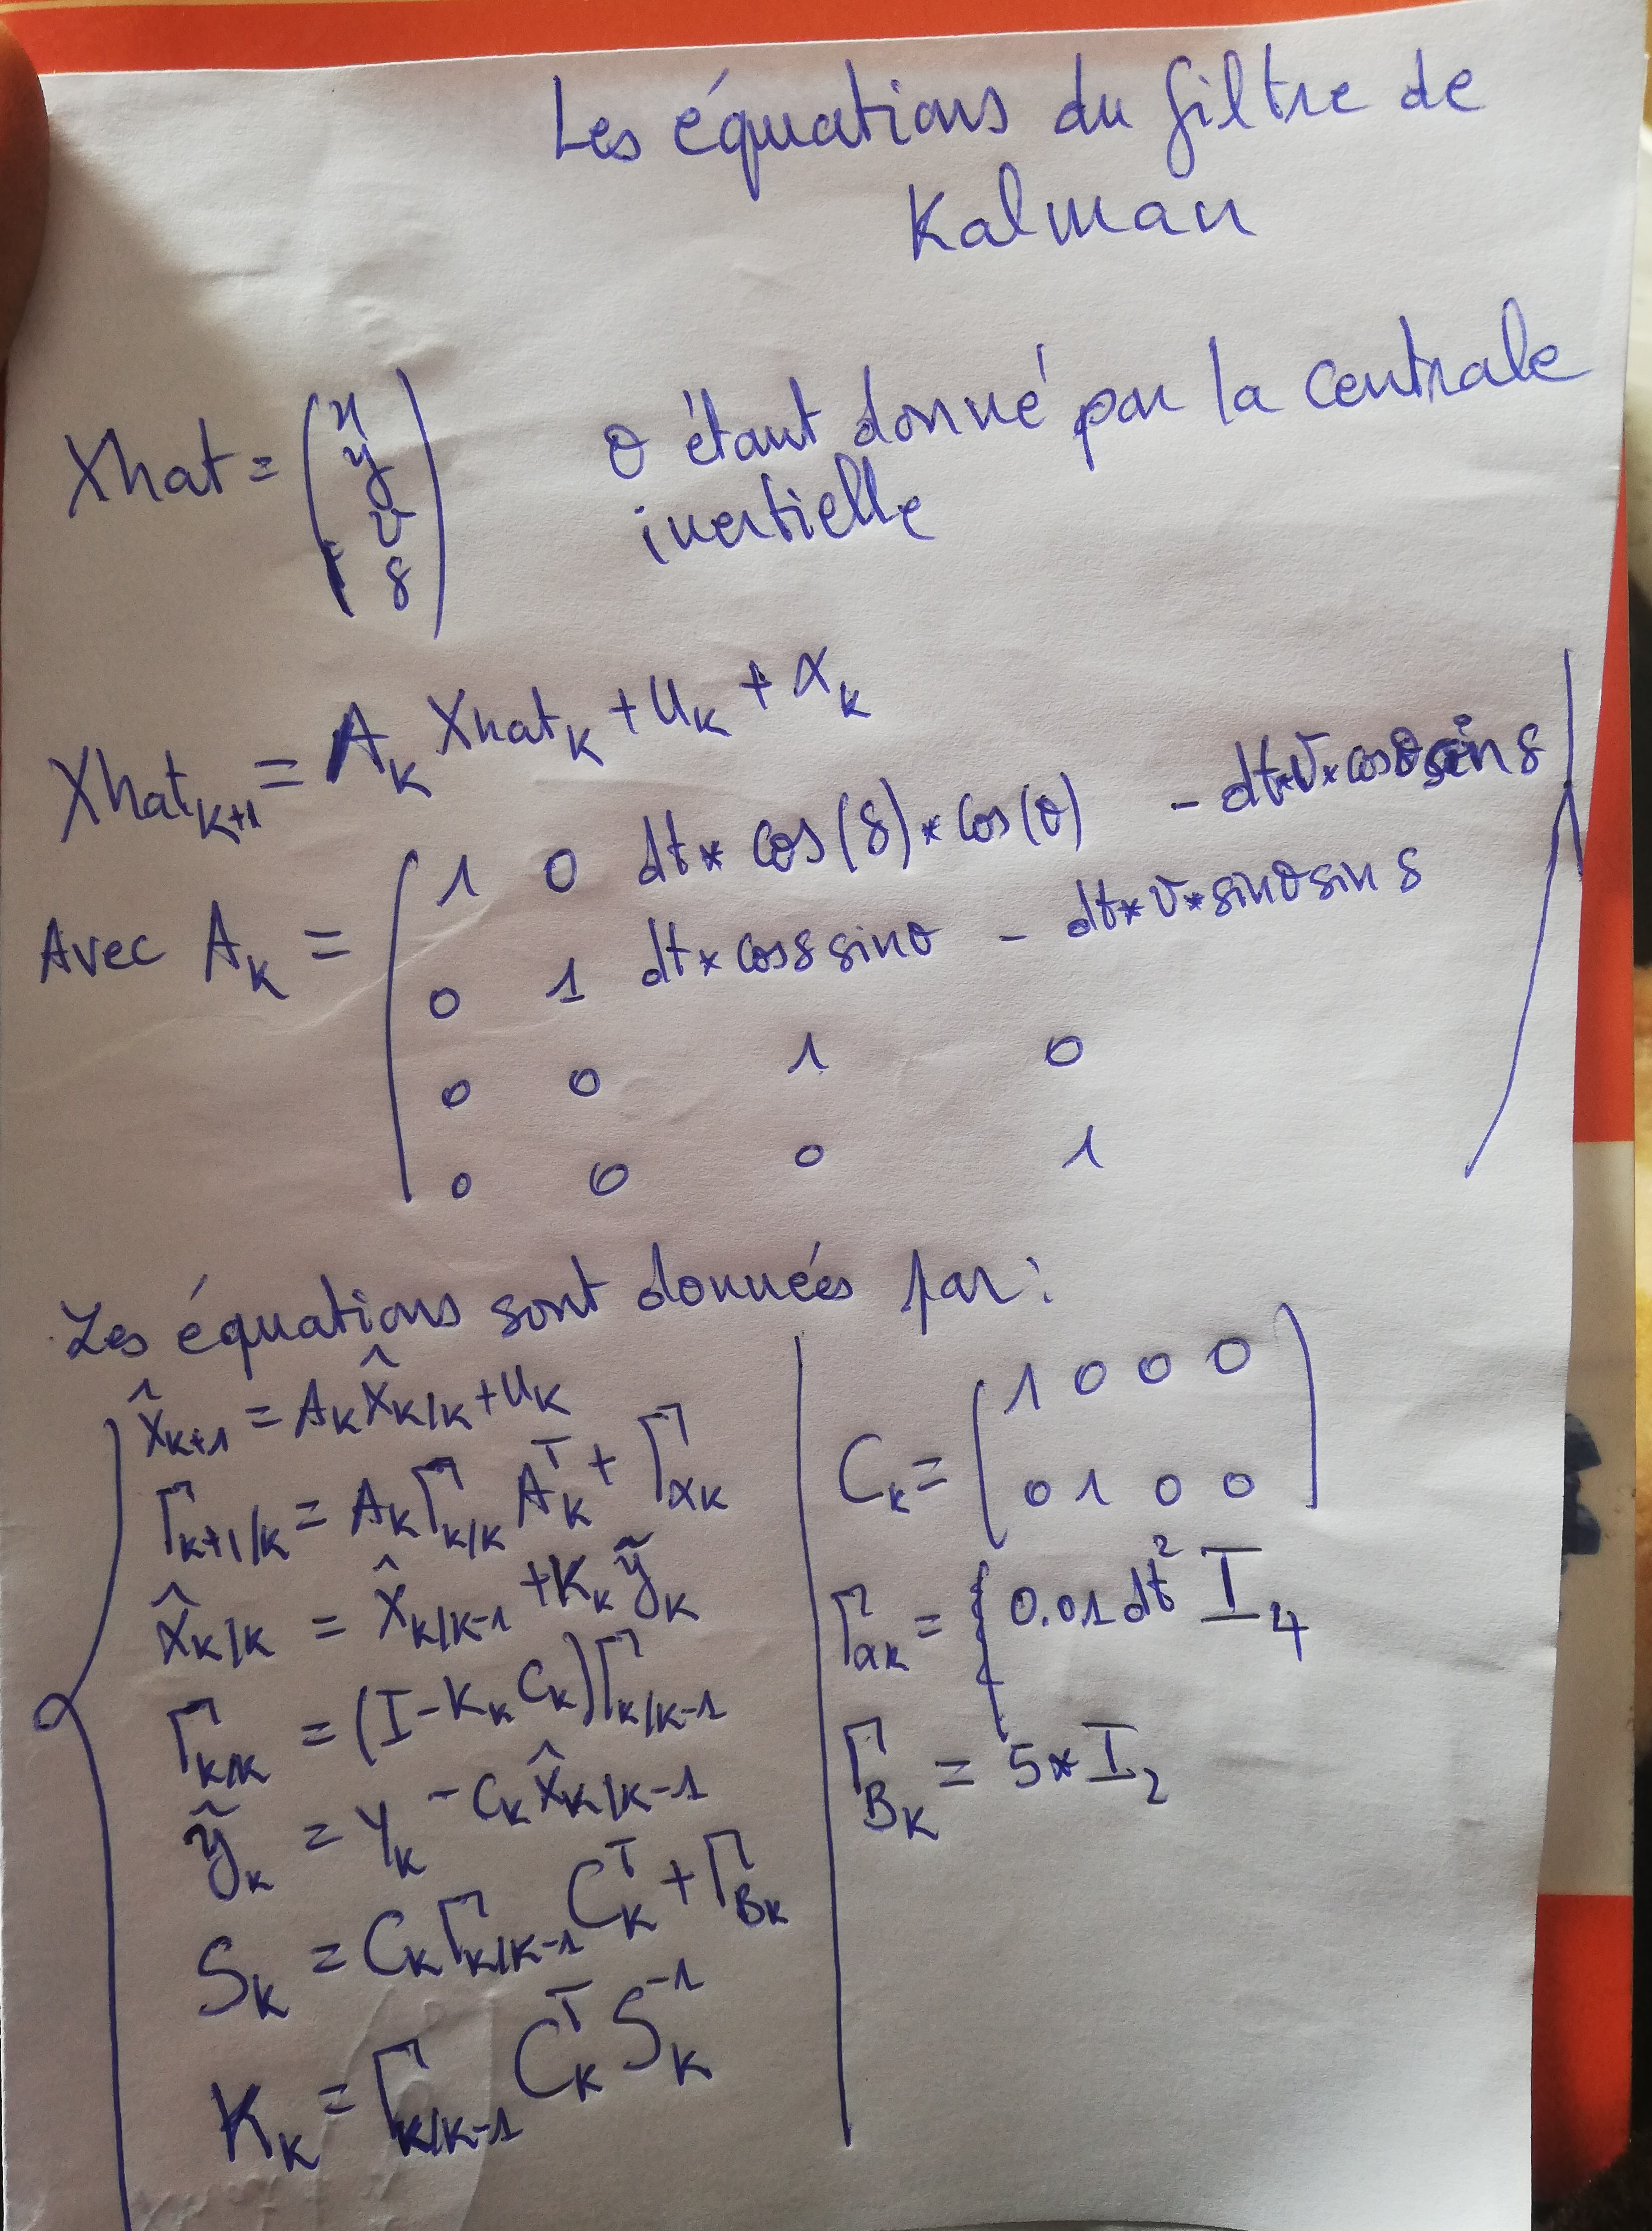
\includegraphics[width=\textwidth]{Images/Equation_filtre_K.jpg}
    \end{center}
    \caption{Kalman Filter Equation}
    \label{fig:Equation}
\end{figure}

